\documentclass{standalone}
\usepackage{tikz}
%\usetikzlibrary{...}
\begin{document}
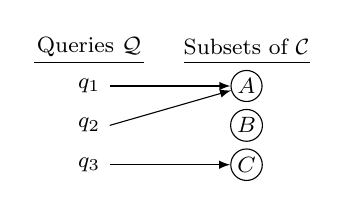
\begin{tikzpicture}
\tikzstyle{every node}=[font=\footnotesize]
\tikzset{>=latex} % arrow heads
\node at (1.0,-0.2) {Queries $\mathcal{Q}$};
\node at (3.0,-0.2) {Subsets of $\mathcal{C}$};
\draw (0.3,-0.4) -- (1.7,-0.4);
\draw (2.2,-0.4) -- (3.8,-0.4);
\node (q1) at (1.0,-0.7) {$q_1$};
\node (q2) at (1.0,-1.2) {$q_2$};
\node (q3) at (1.0,-1.7) {$q_3$};
\node[draw,circle,inner sep=1] (a) at (3.0,-0.7) {$A$};
\node[draw,circle,inner sep=1] (b) at (3.0,-1.2) {$B$};
\node[draw,circle,inner sep=1] (c) at (3.0,-1.7) {$C$};
\draw[->] (q1.east) -- (a);
\draw[->] (q2.east) -- (a);
\draw[->] (q3.east) -- (c);
%\draw[step=1,black!10,very thin] (0,-2) grid (4,0);
\end{tikzpicture}%
\end{document}
